\documentclass[10pt]{article}

\usepackage[T2A]{fontenc}
\usepackage{float}
\usepackage[utf8]{inputenc}
\usepackage[english, russian]{babel}
\usepackage{amsmath}
\usepackage{graphicx}
\usepackage{enumitem}
\usepackage[pdf]{graphviz}
\usepackage{morewrites}
\usepackage{amsfonts}
\DeclareGraphicsExtensions{.pdf,.png,.jpg}

\begin{document}

	{\huge\textbf{Упражение 1}}\\
	{\large
	\begin{enumerate}
		{\Large\item В алфавите $\sum\ =\ \{a,b,c\}$ постройте грамматику для языка $L\ =\ \{\omega\ \in \ \sum^*|\omega\ \text{содержит подстроку} \ aa\}$} \\\\
		
		$S\rightarrow cS\ | \ bS \ | \ aaS_1 \ | \ aS$\\
		$S_1\rightarrow aS_1 \ | \ bS_1 \ | \ cS_1 \ | \ \lambda$\\\\
		
		{\Large\item В алфавите $\sum\ =\ \{a,b,c\}$ постройте грамматику для языка $L\ =\ \{\omega\ \in \ \sum^*|\omega\ \text{не полиндром} \}$} \\\\
		$S\rightarrow aS_1\ | \ bS_2 \ | \ cS_3 $\\
		$S_1\rightarrow S_4b \ | \ S_4c \ | \ Sa $\\
		$S_2\rightarrow S_4a \ | \ S_4c \ | \ Sb $\\
		$S_3\rightarrow S_4a \ | \ S_4b \ | \ Sc $\\
		$S_4\rightarrow aS_1\ | \ bS_2 \ | \ cS_3 \ | \ \lambda$\\\\
		
		{\Large\item В алфавите $\sum\ =\ \{\emptyset,\ \mathbb{N},\ '\{'\ ,\ '\}'\ ,\ ','\ ,\ \cup\}$ постройте грамматику для языка $L\ =\ \{\omega\ \in \ \sum^*|\omega\ - \text{синтаксически}\\ \text{корректная строка обозначающая множество} \}$}\\\\
		$S\rightarrow \emptyset\ | \ \mathbb{N} \ | \ \{S_1\} \ | \  \cup$\\
		$S_1\rightarrow S,S_2 \ | \ S \ | \ \lambda $\\
		$S_2\rightarrow S,S_2 \ | \ S$\\\\
	\end{enumerate}
	{\huge\textbf{Упражение 2}}\\\\
	{\Large В алфавите $\sum\ =\ \{1,+,=\}$ Рассмотрим язык $A=\{1^m+1^n=1^{n+m}|m,n\in\mathbb{N}\}$}\\
	\begin{enumerate}
		{\Large\item Докажите что язык $A$ регулярный (построением) или не регулярный (через лемму о накачке)}\\\\
		 Фиксируем $\forall n=N$ возьмём слово $\alpha=1^N+1^N=1^{2N},\ \alpha \in A,\ |\omega|=4N+2>N $, так как в лемме $|xy|\leq N, \text{как бы мы не взяли } xy,\ y=1^i \implies xy^kz \text{ выходит за пределы языка при } \forall k\neq 1,\text{ так как тогда}\\ \text{в выражении перестаёт выполнятся тождество} \implies$ язык $A$ не регулярный\\
		{\Large\item Постройте КС-грамматику для языка $A$, показывающую, что $A\ -$ контекстно-свободный}\\\\
		$S\rightarrow 1S1\ | \ +S_1 $\\
		$S_1\rightarrow 1S_11 \ | \ = $\\\\
	\end{enumerate}
	{\huge\textbf{Упражение 3}}\\\\
	\begin{enumerate}
			{\Large\item Вы пошли гулять с собакой, ваша собака на поводке длины 2. Это значит что она не может отойти от вас более чем на 2 шага. Пусть  $\sum\ =\ \{h,d\}$, где $h\ -$ ваше перемещение на один шаг вперёд, а $d\ -$ шаг собаки. Прогулка может быть завершена, если собака и человек оказались в одной точке.\\\\
			Пусть $D_1\ =\ \{\omega \ \in \sum^*|\omega \text{ описывает последовательность}\\ \text{ваших шагов и шагов вашей собаки на прогулке с поводком}\}$}
			\begin{enumerate}
				{\Large\item Докажите, что язык $D_1$ регулярный(построением) или не регулярный (через лемму о накачке)}\\
				\digraph{3}\\
				{\Large\item Постройте КС-грамматику для языка $D_1$, показывающую, что $D_1\ -$ контекстно-свободный}\\\\
				$S\rightarrow hS_1\ | \ dS_2 \ | \ \lambda $\\
				$S_1\rightarrow hdS_1 \ | \ dS $\\
				$S_2\rightarrow dhS_2 \ | \ hS $\\\\	
			\end{enumerate}	
			{\Large\item Допустим теперь, что вы также пошли на прогулку с собакой. но не взяли с собой поводок. Это значит, что вы можете отдалится от собаки на любое расстояние.\\\\
			Пусть $D_2\ =\ \{\omega \ \in \sum^*|\omega \text{ описывает последовательность}\\ \text{ваших шагов и шагов вашей собаки на прогулке без поводка}\}$}	
			\begin{enumerate}
				{\Large\item Докажите, что язык $D_2$ регулярный(построением) или не регулярный (через лемму о накачке)}\\\\
				Фиксируем $\forall n=N$ возьмём слово $\alpha=h^Nd^N,\ \alpha \in D_2,\ |\omega|=2N>N $, так как в лемме $|xy|\leq N, \text{как бы мы не взяли } xy,\ y=h^i \implies xy^kz \text{ выходит за пределы языка при } \forall k\neq 1,\text{ так как тогда}\\ \text{в конце прогулки вы и собака окажитесь в разных местах} \implies$ язык $D_2$ не регулярный\\
				{\Large\item Постройте КС-грамматику для языка $D_2$, показывающую, что $D_2\ -$ контекстно-свободный}\\\\
				$S\rightarrow dShS\ | \ hSdS \ | \ \lambda $\\	
			\end{enumerate}		
	\end{enumerate}
	{\huge\textbf{Упражение 4}}\\\\
	{\Large Пусть $Perm(\omega) -$ это множество всех пермутаций строки $\omega$, то есть, множество всех уникальных строк, состоящих из тех же букв и в том же количестве, что и в $\omega$. Если $L\ -$ регулярный язык, то $Perm(L)\ -$ это объединение $Perm(\omega)$ для всех $\omega$ в $L$. Если $L$ регулярный, то $Perm(L)$ иногда тоже регулярный, иногда контекстно-свободный, но не регулярный, а иногда даже не контекстно-свободный.  Рассмотрите следующие регулярные выражения $R$ и установите, является ли $Perm(R)$ регулярным, контекстно-свободным или ни тем и ни другим:}\\\\
	\begin{enumerate}
		{\Large\item $(01)^*$}
		\begin{enumerate}
			\item Фиксируем $\forall n=N$ возьмём слово $\alpha=0^N1^N,\ \alpha \in Perm(R),\ |\omega|=2N>N $, так как в лемме $|xy|\leq N, \text{как бы мы не взяли }\\ xy,\ y=0^i \implies xy^kz \text{ выходит за пределы языка при } \forall k\neq 1,\text{ так как тогда} \text{количество нулей }\neq\text{ количество единиц} \implies\ \alpha\text{ уже не является перестановкой символов в слове}\\ \text{состоящем из пар нулей и единиц}\implies$ язык $Perm(R)$ не регулярный\\
			\item $S\rightarrow 0S1S\ | \ 1S0S \ | \ \lambda $\\
		\end{enumerate}
		{\Large\item $0^*+1^*$}
		\begin{enumerate}
			\item Построим автомат\\ \digraph{4}\\
			\item $S\rightarrow 0S_1\ | \ 1S_2 \ | \ \lambda $\\
			$S_1\rightarrow 0S_1\ | \lambda$\\
			$S_2\rightarrow 1S_2\ | \lambda$\\\\
		\end{enumerate}
		{\Large\item $(012)^*$}
		\begin{enumerate}
			\item Фиксируем $\forall n=N$ возьмём слово $\alpha=0^N1^N2^N,\ \alpha \in Perm(R),\ |\omega|=2N>N $, так как в лемме $|xy|\leq N, \text{как бы мы не взяли }\\ xy,\ y=0^i \implies xy^kz \text{ выходит за пределы языка при } \forall k\neq 1,\text{ так как тогда} \text{количество нулей }\neq\text{ количество единиц и двоек} \implies\ \alpha\text{ уже не является перестановкой символов в слове}\\ \text{состоящем из троек нулей, единиц и двоек}\implies$ язык $Perm(R)$ не регулярный\\
			\item $S\rightarrow 0S1S2S\ | \ 1S0S2S \ |\ 1S2S0S \ | \ 0S2S1S \ |\ 2S1S0S \ |\ 2S0S1S \ | \ \lambda $\\	
		\end{enumerate}
	\end{enumerate}	
	{\huge\textbf{Упражение 5}}\\\\
	\begin{enumerate}
		{\Large\item Пусть грамматика $G -$ праволинейная. Опишите алгоритм построения НКА $N$, такого что $(N)=(G)$. Коротко докажите(от противного),что ваш алгоритм может получить только слова из языка грамматики. Проиллюстрируйте алгоритм на грамматике:\\\\
			$A\rightarrow aB \ | \ bC $\\	
			$B\rightarrow aB \ | \ \lambda $\\
			$C\rightarrow aD \ | \ A \ | \ bC $\\
			$B\rightarrow aD \ | \ bD \ |\ \lambda $\\\\
		}
		Имеем $G\ =\ \langle V,\sum,R,S\rangle$, где\\
		$V\ -$ множество нетерминальных символов\\
		$\sum\ -$ множество терминальных символов\\
		$R\ -$ правила вида $\begin{cases}1.\ A\rightarrow\lambda\\ 2.\ A\rightarrow B\\ 3.\ A\rightarrow aB \end{cases}$\\
		$S\ -$ стартовый нетерминал\\\\
		Тогда НКА $N\ =\ \langle M,Q,y,T,\sigma\rangle$ будет таким:\\
		Мн-во терминальных символов: $M\ = \sum$\\
		Мн-во вершин: $Q\ =\ V$\\
		Стартовая вершина: $y\ =\ s$\\
		Мн-во конечных вершин.: $T=\{t:t\in V,\ \exists\omega\in R: t\rightarrow\lambda\in\omega\}$ \\
		Мн-во переходов $\sigma$ формируем по принципу (относительно номеров из $R$): $\begin{cases}1.\text{ничего}\\ 2.\lambda-\text{переход из }A \text{ в } B\\ 3.\text{переход по } a \text{ из }A \text{ в }B \end{cases}$\\\\
		Докажем $(N)=(G)$\\
		Пусть $x$ не выводится из $G$ , но выводится из $N$\\
		Пусть $x=a_1a_2...a_n\ (a_i \in \sum, \forall i)$\\\\
		При разборе слова автоматом, для каждой буквы $a_i$, мы должны пройти по $\lambda-$переходам из текущей вершины $S$ в вершину $S_1$ из которой есть переход по букве $a_i$, когда буквы закончатся мы аналогично должны дойти до какой то конечной вершины по $\lambda-$переходам.
		Так как в $N$ каждой вершине мы можем поставить в соответствие правило из $G$ (т.к. $Q\ =\ V$) а $\lambda-$переходы между вершинами $A$ и $B$ мы ставили тогда когда в $R$ было правило $A\rightarrow B$ то 
		выходит везде где по $\lambda-$переходам мы добираемся из вершины $S$ в вершину $S_1$, в $G$ $S\Rightarrow^* S_1$, далее так как в $N$ мы ставили переход из $A$ в $B$ по $a$ тогда когда в $R$ было правило $A\rightarrow aB$, значит если в автомате есть переход из $S_1$ в $S_2$ по $a_i$, то в $G$ $S_1\Rightarrow^* a_iS_2$, и наконец так как мы в $N$ обозначали вершину $A$ конечной если в $R$ есть правило $A\rightarrow\lambda$, то если в автомате мы смогли добратся по $\lambda-$переходам из $S_m$ в вершину $S_k$ которая является конечной, значит в $G\ S_m\Rightarrow^* S_k,\ S_k\Rightarrow^* \lambda\ \implies\ S_m\Rightarrow^* \lambda \implies$ $G\Rightarrow^*x\ -$ противоречие.\\\\
		Пусть теперь $x$ выводится из $G$ , но не выводится из $N$\\
		Пусть $x=a_1a_2...a_n\ (a_i \in \sum, \forall i)$\\\\
		Доказывать будем аналогично. Чтобы $y\implies^*a_1S_1$ нужно пройти по переходам вида $A\rightarrow B$ из $y$ в $S$: есть переход $S\rightarrow a_1S_1$, в $N$ можно сделать тоже-самое перейдя по $\lambda-$переходам из $y$ в $S$, а далее из $S$ в $S_1$ по $a_1$, из за принципа построения $N$. Аналогично происходит до конца слова, когда закончатся буквы, допустим на $S_n$, далее $S_n\Rightarrow^*\lambda$, по тем же соображениям мы и в $N$ можем сделать так-же и прийти из $S_n$ в конечную вершину, выходит что если слово выводится из $G$ оно выводится и из $N$.\\\\
		\digraph{5.1}\\\\
		{\Large\item Пусть $N\ -$ НКА. Опишите алгоритм построения КС-грамматики $G$, такой что $(G)=(N)$. Коротко докажите (от противного), что ваш алгоритм может получить только слова из языка НКА. Проиллюстрируйте алгоритм на автомате:}
		\begin{figure}[H]
			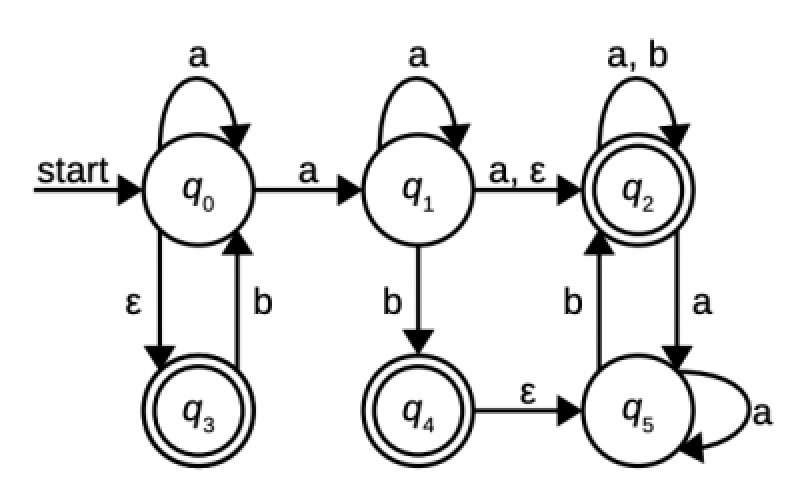
\includegraphics[scale=0.6]{1}
		\end{figure}
		Имеем $N\ =\ \langle M,Q,y,T,\sigma\rangle$, где\\
		$M\ -$ множество терминальных символов\\
		$Q\ -$ множество вершин\\
		$y\ -$ стартовая вершина\\
		$T\ -$ множество конечных вершин\\
		$\sigma\ -$ множество переходов\\\\
		Тогда грамматика $G\ =\ \langle V,\sum,R,S\rangle$ будет такой:\\
		Мн-во нетерминальных символов: $V\ =\ Q$\\
		Мн-во терминальных символов: $\sum\ =\ M$\\
		Стартовый нетерминал: $S\ =\ y$\\
		Мн-во правил вывода $R$ формируем\\по принципу: $\begin{cases} A\rightarrow B\ (\text{есть }\lambda-\text{переход из }A\text{ в }B)\\A\rightarrow aB\ (\text{есть переход по } a\text{ из }A\text{ в }B)\\A\rightarrow\lambda\ (A\ -\text{ терминальная вершина}) \end{cases}$\\\\
		Докажем $(N)=(G)$\\
		Пусть $x$ не выводится из $G$, но выводится из $N$\\
		Пусть $x=a_1a_2...a_n\ (a_i \in \sum, \forall i)$\\\\
		При разборе слова автоматом, для каждой буквы $a_i$, мы должны пройти по $\lambda-$переходам из текущей вершины $S$ в вершину $S_1$ из которой есть переход по букве $a_i$, когда буквы закончатся мы аналогично должны дойти до какой то конечной вершины по $\lambda-$переходам.
		Так как в $N$ каждой вершине мы можем поставить в соответствие правило из $G$ (т.к. $V\ =\ M$) и так как мы создавали правила вида $A\rightarrow B$ когда есть $\lambda-$переход из $A$ в $B$, $S\Rightarrow^*S_1$, так как мы создавали правила вида $A\rightarrow aB$ когда из вершины $A$ есть переход в $B$ по $a$, то $S_1\Rightarrow^*a_iS_2$, аналогично со всеми переходами, теперь если мы можем из вершины $S_n$ перейти в конечную вершину значит $S_n\Rightarrow^*\lambda$, значит $x$ выводится из $G\ -$ противоречие.\\\\
		Пусть теперь $x$ выводится из $G$ , но не выводится из $N$\\
		Пусть $x=a_1a_2...a_n\ (a_i \in \sum, \forall i)$\\\\
		Доказывать будем аналогично. Чтобы $y\Rightarrow^*a_1S_1$ нужно пройти по переходам вида $A\rightarrow B$ из $y$ в $S$: есть переход $S\rightarrow a_1S_1$, в $N$ можно сделать тоже-самое ,так как для каждого подобного правила есть $\lambda-$переход, перейдя по $\lambda-$переходам из $y$ в $S$, а далее из $S$ в $S_1$ по $a_1$, из за принципа построения $N$. Аналогично происходит до конца слова, когда закончатся буквы, допустим на $S_n$, далее $S_n\Rightarrow^*\lambda$, по тем же соображениям мы и в $N$ можем сделать так-же и прийти из $S_n$ в конечную вершину, выходит что если слово выводится из $G$ оно выводится и из $N$.\\\\
		\\\\
		$q_0\rightarrow\ aq_0\ |\ aq_1\ |\ q_3$\\
		$q_1\rightarrow\ aq_1\ |\ bq_4\ |\ aq_2\ |\ q_2$\\
		$q_2\rightarrow\ aq_2\ |\ bq_2\ |\ aq_5$\\
		$q_3\rightarrow\ bq_0\ |\ \lambda$\\
		$q_4\rightarrow\ q_5\ |\ \lambda$\\
		$q_5\rightarrow\ aq_5\ |\ bq_2$
		
	\end{enumerate}	
}
\end{document}
